\begin{tikzpicture}[
    thick,
    font=\small,
    flamesurface/.style={black},
    point/.style={fill=white, draw=black},
    max/.style={fill=mycolor4},
    min/.style={fill=mycolor3},
    infl/.style={fill=mycolor1},
    arrow/.style={-latex, very thick},
    legend line/.style={dash pattern=on 3pt off 3pt, shorten <=1mm},
    legend dark/.style={legend line, black},
    legend light/.style={legend line, dash phase=3pt, white},
]
    % width of the profile plots
    \newlength{\plotwidth}
    \setlength{\plotwidth}{0.4\figurewidth-0.4cm}

    % Scalar field
    \node[anchor=south west, inner sep=0,outer sep=0] (img) at (0, 0) {
        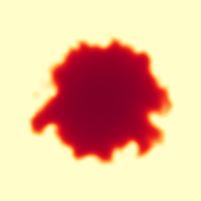
\includegraphics[trim=107 22 20 105,
                         clip,
                         width=0.6\figurewidth]{images/CO2_orig_rdoryl}
    };

    % flame surface and coordinates
    \begin{scope}[
        x={(img.south east)},
        y={(img.north west)},
        shift={(img.south west)}
    ]
        % \draw[help lines, opacity=0.5, xstep=.01,ystep=.01] (0,0) grid (1,1);
        % \draw[help lines,xstep=0.1,ystep=0.1] (0,0) grid (1,1);
        % \foreach \x in {0,...,9} { \node [anchor=north] at (\x/10,0) {0.\x}; }
        % \foreach \y in {0,...,9} { \node [anchor=east] at (0,\y/10) {0.\y}; }

        \draw[flamesurface] plot [smooth] coordinates {
            (0, 0.245)
            (0.04, 0.26)
            (0.06, 0.30)
            (0.08, 0.36)
            (0.1, 0.4)
            (0.14, 0.41)
            (0.19, 0.415)
            (0.23, 0.44)
            (0.27, 0.47)
            (0.31, 0.505)
            (0.36, 0.51)
            (0.4, 0.49)
            (0.425, 0.45)
            (0.435, 0.41)
            (0.435, 0.38)
            (0.445, 0.345)
            (0.49, 0.34)
            (0.535, 0.37)
            (0.575, 0.41)
            (0.61, 0.47)
            (0.63, 0.5)
            (0.67, 0.52)
            (0.71, 0.54)
            (0.73, 0.58)
            (0.725, 0.63)
            (0.7, 0.66)
            (0.62, 0.73)
            (0.585, 0.77)
            (0.565, 0.81)
            (0.56, 0.85)
            (0.575, 0.88)
            (0.61, 0.9)
            (0.67, 0.905)
            (0.715, 0.91)
            (0.76, 0.95)
            (0.79, 1)};


        \coordinate (p1) at (0.04, 0.26);
        \coordinate (p2) at (0.08, 0.36);
        \coordinate (p3) at (0.14, 0.41);
        \coordinate (p4) at (0.23, 0.44);
        \coordinate (p5) at (0.31, 0.505);
        \coordinate (p6) at (0.4, 0.49);
        \coordinate (p7) at (0.435, 0.41);
        \coordinate (p8) at (0.445, 0.345);
        \coordinate (p9) at (0.535, 0.37);
        \coordinate (p10) at (0.61, 0.47);
        \coordinate (p11) at (0.67, 0.52);
        \coordinate (p12) at (0.73, 0.58);
        \coordinate (p13) at (0.7, 0.66);
        \coordinate (p14) at (0.585, 0.77);
        \coordinate (p15) at (0.56, 0.85);
        \coordinate (p16) at (0.61, 0.9);
        \coordinate (p17) at (0.715, 0.91);

    \end{scope}

    % profile for point 1
    \begin{scope}[
            shift={($(img.south east)!0.66!(img.north east) + (0.3cm, 0.4cm)$)},
            x={\plotwidth},
            y={0.15\figurewidth}
        ]
        \coordinate (pl1) at (0, 0);
        \draw[arrow] (0, 0) -- (1, 0) node [below] {$t$};
        \draw[point] (0.5, 0) circle (0.8mm) node [below] {$\vp_1$};
        \draw[-latex] (0, 0) -- (0, 1)
            node[right, yshift=1mm] {\ce{CO2}};
        \draw (0, 0.9) to[out=0, in=130]
              (0.5, 0.5) to[out=-50, in=180]
              (0.75, 0) --
              (0.9, 0) to[out=0, in=200]
              (1, 0.1);
        \draw[point, infl] (0.5, 0.5) circle (0.8mm);
        \draw[point, max] (0, 0.9) circle (0.8mm);
        \draw[point, min] (0.75, 0.0) circle (0.8mm);
    \end{scope}

    % profile for point 2
    \begin{scope}[
            shift={($(img.south east)!0.33!(img.north east) + (0.3cm, 0.4cm)$)},
            x={\plotwidth},
            y={0.15\figurewidth}
        ]
        \coordinate (pl2) at (0, 0);
        \draw[arrow] (0, 0) -- (1, 0) node [below] {$t$};
        \draw[point] (0.5, 0) circle (0.8mm) node [below] {$\vp_2$};
        \draw[-latex] (0, 0) -- (0, 1)
            node[right, yshift=1mm] {\ce{CO2}};
        \draw (0, 0.75) to[out=-5, in=140]
              (0.5, 0.5) to[out=-40, in=180]
              (0.8, 0) --
              (1, 0);
        \draw[point, infl] (0.5, 0.5) circle (0.8mm);
        \draw[point, max] (0, 0.75) circle (0.8mm);
        \draw[point, min] (0.8, 0.0) circle (0.8mm);
    \end{scope}

    % profile for point 3
    % \begin{scope}[
    %         shift={($(img.south east)!0.00!(img.north east) + (0.3cm, 0.4cm)$)},
    %         x={\plotwidth},
    %         y={0.15\figurewidth}
    %     ]
    %     \coordinate (pl3) at (0, 0);
    %     \draw[arrow] (0, 0) -- (1, 0);
    %     \draw[point] (0.5, 0) circle (0.8mm) node [below] {$\vp_3$};
    %     \draw[-latex] (0, 0) -- (0, 1)
    %         node[right, yshift=1mm] {\ce{CO2}};
    %     \draw (0, 0.75) to[out=10, in=180]
    %           (0.25, 0.85) to[out=0, in=130]
    %           (0.5, 0.5) to[out=-50, in=180]
    %           (0.8, 0) --
    %           (1, 0);
    %     \draw[point, infl] (0.5, 0.5) circle (0.8mm);
    %     \draw[point, max] (0.25, 0.85) circle (0.8mm);
    %     \draw[point, min] (0.8, 0.0) circle (0.8mm);
    % \end{scope}
    \begin{scope}[
            shift={($(img.south east)!0.00!(img.north east) + (0.3cm, 0.4cm)$)},
            x={\plotwidth},
            y={0.15\figurewidth}
        ]
        \coordinate (pl3) at (0, 0);
        \draw[arrow] (0, 0) -- (1, 0) node [below] {$t$};
        \draw[point] (0.5, 0) circle (0.8mm) node [below] {$\vp_3$};
        \draw[-latex] (0, 0) -- (0, 1)
            node[right, yshift=1mm] {\ce{CO2}};
        \draw (0, 0.47) to[out=40, in=180]
              (0.3, 0.75) to[out=0, in=130]
              (0.5, 0.5) to[out=-50, in=180]
              (0.8, 0) --
              (1, 0);
        \draw[point, infl] (0.5, 0.5) circle (0.8mm);
        \draw[point, max] (0.3, 0.75) circle (0.8mm);
        \draw[point, min] (0.8, 0.0) circle (0.8mm);
    \end{scope}

    % arrows
    \begin{scope}
        \clip (img.south east) rectangle (img.north west);

        \draw[arrow] (p1) -- +(130:1.2cm) -- +(310:1.2cm);
        \draw[arrow] (p2) -- +(155:1.2cm) -- +(335:1.2cm);
        \draw[arrow] (p3) -- +(93:1.2cm) -- +(273:1.2cm);
        \draw[arrow] (p4) -- +(125:1.2cm) -- +(305:1.2cm);
        \draw[arrow] (p5) -- +(105:1.2cm) -- +(285:1.2cm);
        \draw[arrow] (p6) -- +(55:1.2cm) -- +(235:1.2cm);
        \draw[arrow] (p7) -- +(7:1.2cm) -- +(187:1.2cm); %
        \draw[arrow] (p8) -- +(60:1.2cm) -- +(240:1.2cm);
        \draw[arrow] (p9) -- +(130:1.2cm) -- +(310:1.2cm);
        \draw[arrow] (p10) -- +(145:1.2cm) -- +(325:1.2cm);
        \draw[arrow] (p11) -- +(115:1.2cm) -- +(295:1.2cm);
        \draw[arrow] (p12) -- +(175:1.2cm) -- +(355:1.2cm); %
        \draw[arrow] (p13) -- +(230:1.2cm) -- +(50:1.2cm);
        \draw[arrow] (p14) -- +(215:1.2cm) -- +(35:1.2cm); %
        \draw[arrow] (p15) -- +(165:1.2cm) -- +(345:1.2cm);
        \draw[arrow] (p16) -- +(100:1.2cm) -- +(280:1.2cm);
        \draw[arrow] (p17) -- +(125:1.2cm) -- +(305:1.2cm);
    \end{scope}

    % color bar
    \node[draw=black,
          inner sep=0.05mm,
          below right=0.3cm and 0.3cm of img.north west] (cscale) {
        \rotatebox{-90}{%
            
\includegraphics[width=2.5cm, height=0.25cm]{figures/rdoryl.png}%
        }
    };
    \node[anchor=south west, inner sep=0, outer sep=0, xshift=1mm] at (cscale.south east) {
        \small min
    };
    \node[anchor=north west, inner sep=0, outer sep=0, xshift=1mm] at (cscale.north east) {
        \small max
    };
    \node[anchor=north] at (cscale.south) {\small \ce{CO2}};

    % points
    \foreach \i in {1,...,17} {
        \draw[point] (p\i) circle (0.8mm);
    }

    % marking circles
    \begin{scope}[
        x={(img.south east)},
        y={(img.north west)},
        shift={(img.south west)}
    ]
        \draw[mycolor1, very thick] (0.48, 0.385) circle (0.6cm);
        \draw[mycolor1, very thick, rotate around={-43: ($(p13)!0.5!(p14)$)}]
            ($(p13)!0.5!(p14)$) circle (0.78cm and 0.25cm);
    \end{scope}


    % profile plot connecting lines
    \draw[legend dark] (p14) |- (pl1);
    \draw[legend dark] (p12) |- (pl2);
    % \draw[legend dark] (p9) |- (pl3);
    \draw[legend dark] (p7) |- (pl3);

    % \draw[legend light] (p14) |- (pl1);
    % \draw[legend light] (p12) |- (pl2);
    % \draw[legend light] (p9) |- (pl3);

    % point labels
    \node[above left=-0.1cm and 0.05cm of p14] {$\vp_1$};
    \node[above right=-0.05cm and -0.07cm of p12] {$\vp_2$};
    % \node[right=0.1cm of p9] {$\vp_3$};
    \node[above left=-0.1cm and -0.05cm of p7] {$\vp_3$};
\end{tikzpicture}%